\section{Experiments}\label{sec:exp}

%\begin{figure}[!h]
%\centering
%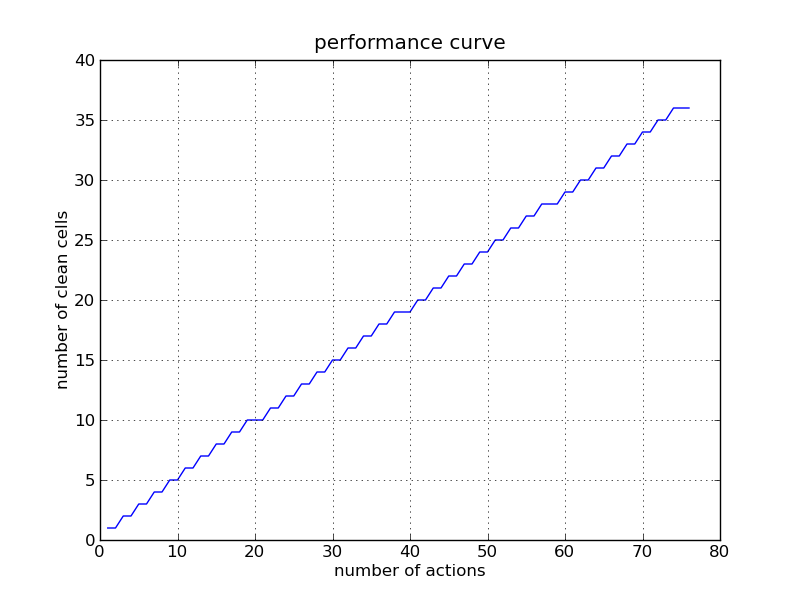
\includegraphics[scale=.35]{img/agent1.png}
%\caption{Performance of Memoryless Deterministic Agent}
%\label{fig:agent1}
%\end{figure}

%\begin{table}[h]
%    \centering
%    \begin{tabular}{|l|c|c|c|c|c|c|c|c|c|c|}
%        \hline
%        trials 1-10 & 495 & 625 & 514 & 647 & 842 & 614 & 550 & 532 & 532 & 924\\ \hline
%        trials 11-20 & 510 & 585 & 519 & 616 & 504 & 434 & 477 & 538 & 489 & 479\\ \hline
%        trials 21-30 & 385 & 562 & 531 & 591 & 551 & 458 & 515 & 711 & 662 & 439\\ \hline
%        trials 31-40 & 461 & 398 & 604 & 601 & 900 & 428 & 507 & 594 & 512 & 735\\ \hline
%        trials 41-50 & 572 & 574 & 490 & 498 & 578 & 517 & 380 & 444 & 605 & 506\\ \hline
%    \end{tabular}
%    \caption{Number of actions to take to clean $90\%$ of the room}\label{tab:agent2}
%\end{table}

%\begin{figure}[!h]
%        \centering
%        \subfloat[Number of actions]{
%                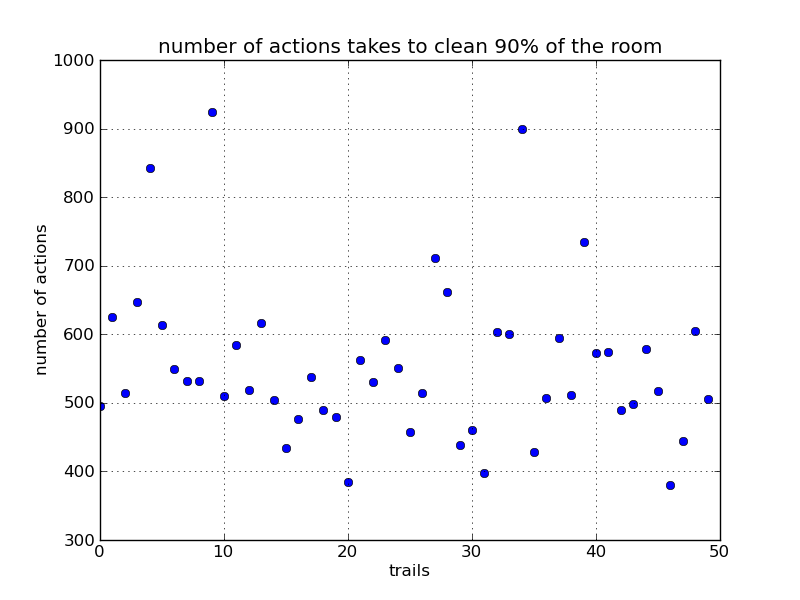
\includegraphics[scale=0.35]{img/num_actions.png}
%        }
%        \hspace{0.5in}
%        \subfloat[Performance curves]{
%                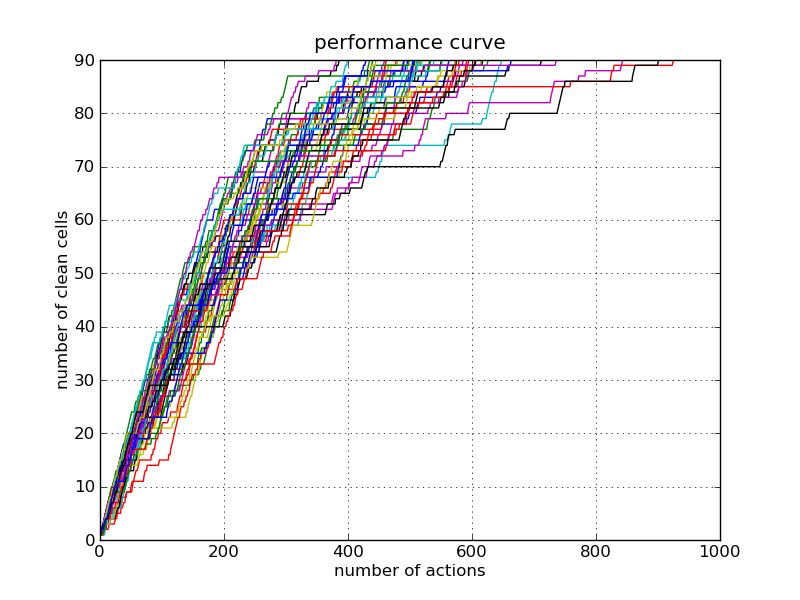
\includegraphics[scale=0.35]{img/rand.png}
%        }
%        \caption{Performance of randomized reflex agent}\label{fig:agent2}
%\end{figure}

\subsection{Heuristics}
We observed that the length of a path is the steps moving from initial state to goal state. So a natural heuristic can be designed based on an optimistic estimation of how many steps need to turn a state to its final goal. The first admissible heuristic is as following:
\[
h(s) = (\sum_i |s(1,i)-i| ) + numberDisks(s(2)) + numberDisks(s(3))
\]
Here, s(i,j) is the $jth$ disks in peg $i$. The intuition is that for a disk $k$ in peg $1$, it has to take $|k-i|$ steps to get to the place it should be, where $i$ is its current location on the peg. For example, if the $9th$ disk is on the bottom, it has to take $9-0$ steps to get to the top. For disks on peg $2$ and peg $3$, they have to be moved from the current location to peg $1$ in at least $1$ step. This is in fact an admissible heuristic. A simple justification is given as
follows: for any disk on peg $1$, before it reaches its ideal position, there should be $|k-i|$ disks put underneath it, and for every such disk, it takes at least one step. Of course, a much trivial admissible heuristic can be used here, such as number of disks in the first peg, but for computational efficiency, we choose this admissible heuristic in our experiment.

For non-admissible heuristic, we simplily enlarge the admissible heuristic by a factor of $2$. This is also reasonable since before we move a disk to its ideal position, usually we have to move another disk out of that place, which makes the number of steps double. But obviously this is not ture for all the cases. We can give a counterexample easily. 
\[
h(s) = 2 \times [(\sum_i |s(1,i)-i| ) + numberDisks(s(2)) + numberDisks(s(3))]
\]

\subsection{Results}

\begin{figure}[!t]
\centering
\begin{tabular}{cc}
\subfloat[A* nodes: all 140 experiments]{\includegraphics[scale=0.32]{img/tnode_Astar.pdf}} 
   & \subfloat[RBFS nodes: all 140 experiments]{\includegraphics[scale=0.32]{./img/tnode_RBFS.pdf}}\\
\subfloat[A* average searched nodes]{\includegraphics[scale=0.32]{./img/anode_Astar.pdf}} 
   & \subfloat[RBFS average searched nodes]{\includegraphics[scale=0.32]{./img/anode_RBFS.pdf}}\\
%\subfloat[E]{\includegraphics[width=2cm]{logo}} 
%   & \subfloat[F]{\includegraphics[width=3cm]{logo}}\\
\end{tabular}
\caption{Plots for the number of nodes searched against the problem size for each algorithm and heuristic. For the first 2 figures, number of disks within 4-10, every 20 examples have the same problem size. We show average expanded nodes against number of disks for a clear demonstration. As the problem size becomes larger, the number of searched nodes grow up exponentially.}
\label{fig:nodes}
\end{figure}

\begin{figure}[!t]
\centering
\begin{tabular}{cc}
\subfloat[A*: average cpu time (s) on heuristics]{\includegraphics[scale=0.32]{./img/AHcpu-aver.pdf}} 
   & \subfloat[RBFS: average cpu time (s) on heuristics]{\includegraphics[scale=0.32]{./img/RHcpu-aver.pdf}}\\
\subfloat[A*: average cpu time (s) on whole problem]{\includegraphics[scale=0.32]{./img/ATcpu-aver.pdf}} 
   & \subfloat[RBFS: average cpu time (s) on whole problem]{\includegraphics[scale=0.32]{./img/RTcpu-aver.pdf}}\\
%\subfloat[E]{\includegraphics[width=2cm]{logo}} 
%   & \subfloat[F]{\includegraphics[width=3cm]{logo}}\\
\end{tabular}
\caption{Plots for the average cpu time against the problem size over 20 examples for each algorithm and heuristic.}
\label{fig:cputime}
\end{figure}

\begin{figure}[!t]
\centering
\begin{tabular}{cc}
\subfloat[Nodes against disks for admissible heurisitic]{\includegraphics[scale=0.32]{../results/node_Astar_RBFS_H_ad.pdf}} 
   & \subfloat[Nodes against disks for non-admissible heurisitic]{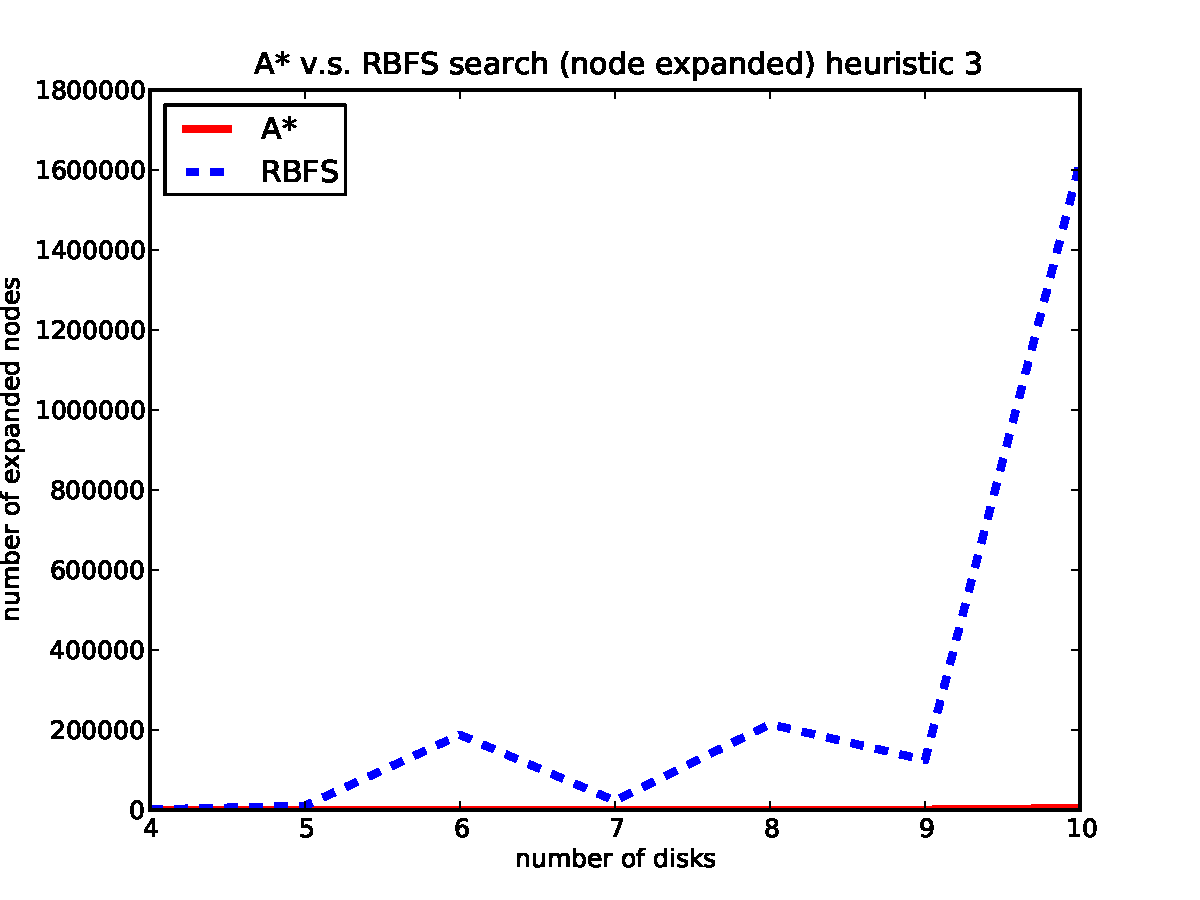
\includegraphics[scale=0.32]{../results/node_Astar_RBFS_H_nad.pdf}}\\
%\subfloat[cpu time against disks for heurisitic 1]{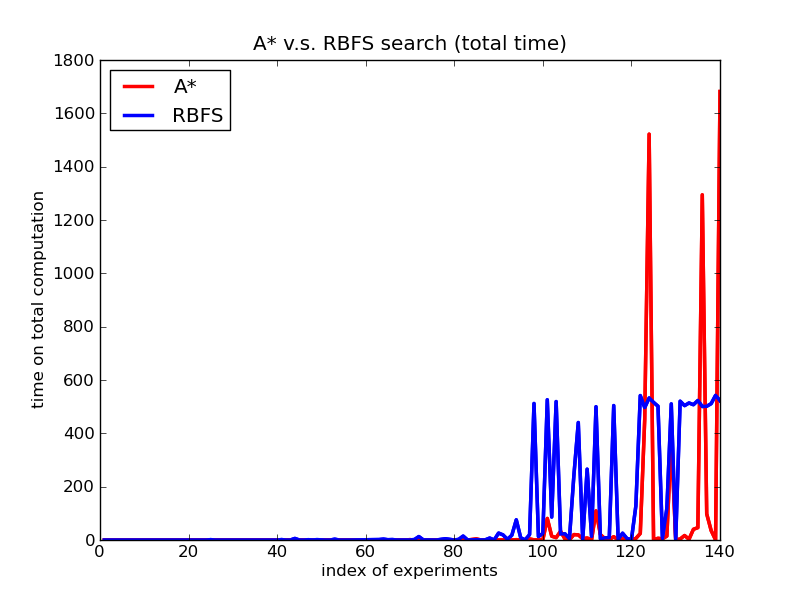
\includegraphics[scale=0.32]{../results/Astar_RBFS_H1_cpu.png}} 
   %& \subfloat[cpu time against disks for heurisitic 2]{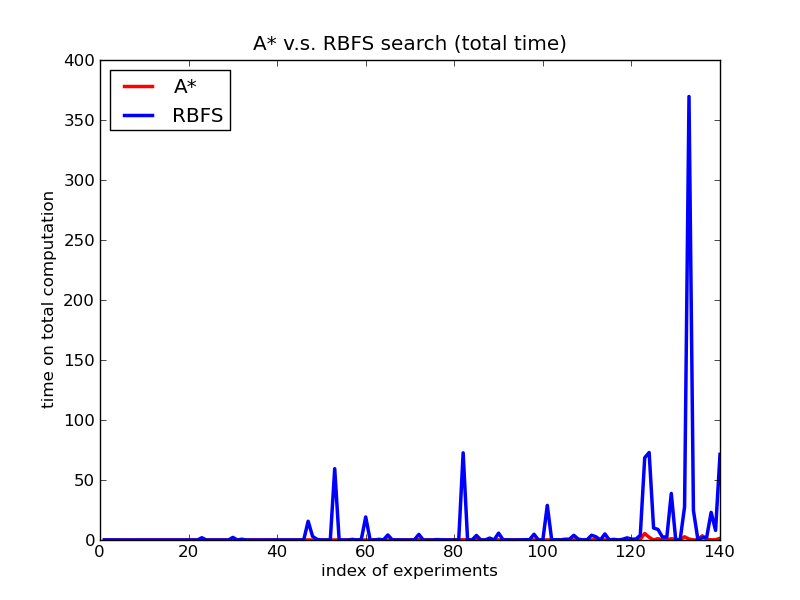
\includegraphics[scale=0.32]{../results/Astar_RBFS_H2_cpu.png}}\\
\end{tabular}
\caption{Performance comparisons between A* and RBFS}
\label{fig:astar-rbfs}
\end{figure}

\begin{table}[!h]
    \centering
    \scalebox{0.9}{
	    \begin{tabular}{|l|c|c|c|c|c|c|c|}
		\hline
		Disks: & 4 & 5 & 6 & 7 & 8 & 9 & 10\\ \hline
		A*/admissible & 8.8 & 11.6 & 13.95 & 16.5 & 18.2 & n/a & n/a\\ \hline
		%A*/admissible H7 & 8.95 & 11.6 & 13.95 & 16.75 & 19.2 & 22.4 & 24.77\\ \hline
		RBFS/admissible & 8.8 & 11.6 & 13.95 & 16.35 & 17.11 & n/a & n/a\\ \hline
		A*/nonadmissible 1 & 8.85 & 11.85 & 14.6 & 17.5 & 20.2 & 24.1 & 27.6\\ \hline
		RBFS/nonadmissible 1 & 8.85 & 11.85 & 15.25 & 19 & 22.21 & 26.81 & 32.25 \\ \hline
		A*/nonadmissible 2 & 9.25 & 12.95 & 16.5 & 20.05 & 23.8 & 27.4 & 34.05\\ \hline
		RBFS/nonadmissible 2 & 11.25 & 17.85 & 24.35 & 32.75 & 40.35 & 50.7 & 64.55\\ \hline
	    \end{tabular}
    }
    \caption{Average solution length per algorithm, heuristic and disk size. n/a means unable to compute within 10 minutes for all problems.}\label{tab:solen}
\end{table}


